% This is "sig-alternate.tex" V1.9 April 2009
% This file should be compiled with V2.4 of "sig-alternate.cls" April 2009
%
% This example file demonstrates the use of the 'sig-alternate.cls'
% V2.4 LaTeX2e document class file. It is for those submitting
% articles to ACM Conference Proceedings WHO DO NOT WISH TO
% STRICTLY ADHERE TO THE SIGS (PUBS-BOARD-ENDORSED) STYLE.
% The 'sig-alternate.cls' file will produce a similar-looking,
% albeit, 'tighter' paper resulting in, invariably, fewer pages.
%
% ----------------------------------------------------------------------------------------------------------------
% This .tex file (and associated .cls V2.4) produces:
%       1) The Permission Statement
%       2) The Conference (location) Info information
%       3) The Copyright Line with ACM data
%       4) NO page numbers
%
% as against the acm_proc_article-sp.cls file which
% DOES NOT produce 1) thru' 3) above.
%
% Using 'sig-alternate.cls' you have control, however, from within
% the source .tex file, over both the CopyrightYear
% (defaulted to 200X) and the ACM Copyright Data
% (defaulted to X-XXXXX-XX-X/XX/XX).
% e.g.
% \CopyrightYear{2007} will cause 2007 to appear in the copyright line.
% \crdata{0-12345-67-8/90/12} will cause 0-12345-67-8/90/12 to appear in the copyright line.
%
% ---------------------------------------------------------------------------------------------------------------
% This .tex source is an example which *does* use
% the .bib file (from which the .bbl file % is produced).
% REMEMBER HOWEVER: After having produced the .bbl file,
% and prior to final submission, you *NEED* to 'insert'
% your .bbl file into your source .tex file so as to provide
% ONE 'self-contained' source file.
%
% ================= IF YOU HAVE QUESTIONS =======================
% Questions regarding the SIGS styles, SIGS policies and
% procedures, Conferences etc. should be sent to
% Adrienne Griscti (griscti@acm.org)
%
% Technical questions _only_ to
% Gerald Murray (murray@hq.acm.org)
% ===============================================================
%
% For tracking purposes - this is V1.9 - April 2009

\documentclass{sig-alternate}
  \pdfpagewidth=8.5truein
  \pdfpageheight=11truein
 \usepackage{graphicx}
 \usepackage{xcolor}
 \usepackage{makecell}
 \usepackage[table]{colortbl}
 \usepackage[hyphens]{url}
\usepackage{hyperref}
\usepackage{breakurl}
\usepackage{listings}
\usepackage{acronym}
\begin{document}
%
% --- Author Metadata here ---
\conferenceinfo{15th AmiEs}{September 22-24th, 2016, Heraklion, Crete/Greece}
\CopyrightYear{2016} % Allows default copyright year (2002) to be over-ridden - IF NEED BE.
\crdata{978-1-4503-3196-8/15/04}  % Allows default copyright data (X-XXXXX-XX-X/XX/XX) to be over-ridden.
% --- End of Author Metadata ---

\title{An Insight to Cracking Solutions and Circumvention of Major Protection Methods for Android}



%
% You need the command \numberofauthors to handle the 'placement
% and alignment' of the authors beneath the title.
%
% For aesthetic reasons, we recommend 'three authors at a time'
% i.e. three 'name/affiliation blocks' be placed beneath the title.
%
% NOTE: You are NOT restricted in how many 'rows' of
% "name/affiliations" may appear. We just ask that you restrict
% the number of 'columns' to three.
%
% Because of the available 'opening page real-estate'
% we ask you to refrain from putting more than six authors
% (two rows with three columns) beneath the article title.
% More than six makes the first-page appear very cluttered indeed.
%
% Use the \alignauthor commands to handle the names
% and affiliations for an 'aesthetic maximum' of six authors.
% Add names, affiliations, addresses for
% the seventh etc. author(s) as the argument for the
% \additionalauthors command.
% These 'additional authors' will be output/set for you
% without further effort on your part as the last section in
% the body of your article BEFORE References or any Appendices.

\numberofauthors{4} %  in this sample file, there are a *total*
% of EIGHT authors. SIX appear on the 'first-page' (for formatting
% reasons) and the remaining two appear in the \additionalauthors section.
%
\author{
% You can go ahead and credit any number of authors here,
% e.g. one 'row of three' or two rows (consisting of one row of three
% and a second row of one, two or three).
%
% The command \alignauthor (no curly braces needed) should
% precede each author name, affiliation/snail-mail address and
% e-mail address. Additionally, tag each line of
% affiliation/address with \affaddr, and tag the
% e-mail address with \email.
%
% 1st. author
\alignauthor Nils Kannengiesser\\
       \affaddr{Technical University of Munich}\\
       \affaddr{Division for Operating Systems, Faculty of Informatics}\\
       \affaddr{Munich, Germany}\\
       \email{nils.kannengiesser@tum.de }
% 2nd. author
\alignauthor Johannes Neutze\\
       \affaddr{Technical University of Munich}\\
       \affaddr{Division for Operating Systems, Faculty of Informatics}\\
       \affaddr{Munich, Germany}\\
       \email{neutze@mytum.de}
% 3rd. author
\alignauthor Uwe Baumgarten\\
       \affaddr{Technical University of Munich}\\
       \affaddr{Division for Operating Systems, Faculty of Informatics}\\
       \affaddr{Munich, Germany}\\
       \email{baumgaru@in.tum.de}
           \and 
 % use '\and' if you need 'another row' of author names
% 4th. author
\alignauthor Sejun Song\\
       \affaddr{University of Missouri}\\
       \affaddr{Kansas City, Kansas, USA}\\
       \email{sjsong@umkc.edu}
}



\maketitle
\begin{abstract}

Android is a target of software piracy.
Application stores are trying to counteract piracy attempts by providing license verification libraries but even those do not stop theft of intellectual property.
The scope of this paper is to present different attack methods.
Insights to the attacks can be used to create countermeasures that are addressed shortly, while presenting their details in a different paper (available at this conference) instead.
\end{abstract}


% A category with the (minimum) three required fields
\category{K.6.5}{Security and Protection}{Unauthorized access}

\terms{SECURITY}

\keywords{Android, Google, Amazon, LVL, DRM, Copy Protection, Attacks}



\section{INTRODUCTION}

In recent years, a new operating system hit the market and depending on the country viewed, has reached market shares of up to 90\% \cite{AT2}. Its name? Android. While initially intended for smart-phones only, Android is now available on all kinds of devices like tablets, watches or even smart-TVs. With such a large market share comes a great responsibility to protect intellectual property, but unfortunately protecting apps and content was never a high priority on Android \cite{nils}. There is no obvious reason why the protection has not been improved since 2010, when Android's License Verification Library (LVL) was released and soon after, cracked \cite{AT1}. Google likes to transfer the burden of improving security to its developers by stating "The security of your application's licensing controls ultimately relies on the design of your implementation itself." \cite{lvlOverview}. Instead, Amazon uses a different approach by injecting their protection into an app at the developer's request during the upload to the market \cite{AT3}. While this approach is much more developer friendly, their security solution is not much more secure either. Here the reasons are the fundamental issues of Android in terms of the easy reengineering of apps that lies in the responsibility of Google \cite{nils}.
While the main purpose of this paper is to present the known attack options on protections used by common markets, it also covers the details of one of the most widely used cracking tools, "Lucky Patcher" \cite{luckypatcherPage}, analyzed by us in detail. In addition and to underline our intention as security researchers, a brief summary is given to possible protection topics, while further details are addressed in a different paper \footnote{Title:"Securing License Verification by using Native Code, Fusing Options and Indirect Method Triggering on Android"} available at this conference as well.

\section{BACKGROUND}

\subsection{Lucky Patcher}
Lucky Patcher is an Android cracking application with various functionalities.
This includes basic features, such as creating backups or restoring applications, and more advanced features that include modifying the code of applications.
Lucky Patcher allows the changing of application permissions, removal of advertisements and the circumventing of license verification mechanisms.
Some of these features require the device to be rooted.
Applying features on an application does not change the functionality of the target application but voids the license verification.
Success is not guaranteed, i.e. some applications are resistant to cracking.
The current version of the application, 6.2.4, can be downloaded for free on a dedicated website \cite{luckypatcherPage}.

\subsection{Reengineering Tools}
Besides the tools available to non-skilled users to perform the cracking of apps, more advanced users, researchers and security experts can rely on tools like the APKtool \cite{apktool} used to disassemble any Android application available in the form of an APK file. The resulting assembly dialect is called smali code and may be described as a high-level assembly code. Modifications of the smali code are easily made and APKs reconstructed, signed and used as usual.

Alternatives to the APKtool are the use of usual Java decompilers that require the embedded DEX file after it has been converted to a JAR file. The benefit of having Java code, in comparison to smali-code, is that it is even easier to understand the program logic, although the reengineered code is often quite poor \cite{nils}.

\subsection{Java Code Interception (Xposed Framework) }
The "Xposed Framework" \cite{AT4} was developed a few years ago and allows modification of Android application on-the-fly by intercepting methods before and after these functions are executed. The interception is done by injecting the required library into the so-called Zygote process that is forked for any newly started Android app and therefore always present in new applications to allow the interception of any (Java) methods \cite{AT4}.

\subsection{Native Code Interception (LD\_PRELOAD etc.) }

Intercepting native code is also possible, although it is more difficult in comparison to the interception of Java code. While there have been frameworks available in the past, like "Cydia Substrate" \cite{AT5} that cannot be used with Android versions after 4.3, a remaining option might be "Frida" \cite{AT6} that uses JavaScript for control. An even easier approach could be to replace a function, when a method name is known using LD\_PRELOAD directive as shown in \cite{AT8}. Replacing a function using that directive seems to work even on recent Android versions (6.0.1) \cite{nils}.

\subsection{Typical App Protections}
This section introduces the common protection methods. The License Verification Library (LVL) by Google, the injected Amazon DRM in their related Appstore and examples for third party protections.

\subsubsection{License Verification Library}
Google introduced the LVL back in 2010 as a tool to fight piracy of applications \cite{lvlRelease}.
It is a simple solution for developers used to verify users against applications purchased on Google Play Store.
The LVL library provides the implementation of the verification while leaving full control over handling the result to the developer.
The library is based on a network service which queries the trusted Google Play license servers to validate whether the user has purchased the application.
Since the source code is provided as part of the Android SDK, the developer just has to implement  the actions to be taken when the response is returned.
Google suggests to modify the library to create a unique implementation that is less vulnerable to code cracking attacks \cite{lvlOverview}\cite{lvlSetup}. 
The classes are the LicenseValidator class, which is responsible for decrypting and verifying the server's response. The policy classes for storing the response, namely APKExpansionPolicy class and ServerManagedPolicy class, which are provided by Google.
The LicenseChecker class is repsonsible for initiating the license check and the ILicenseResultListener class, which provides the interface for verifying the license \cite{addingLvl}.\\

\subsubsection{Amazon DRM}

Amazon uses a different approach to protect developer's apps in their Appstore by using a technique to inject code into these apps. Here, it does not matter if the app actually uses the DRM protection; Amazon's libraries are injected anyway even if the protection will not be activated. Amazon points out that this approach is required to interact with their App-Store app \cite{AT3}. \\

\subsubsection{Other protections}

Besides the widely known protection mechanisms, other markets like SlideMe provide their own license verifications that have similarities to Google's LVL \cite{AT7}. Furthermore, there are various protections by other researchers available, but none of them seem to be used widely or are recommend by Google or Amazon. Examples to be mentioned are the solution using smart-cards and encryption of the application as presented by Shoaib et al. \cite{RW1}. Another option is the solution approach called "DIVILAR" by Wu Zhou et al. \cite{RW3} introducing a virtual machine protection for older Android versions. In addition, protections using dongles that can execute code in a secure manner could be developed using \cite{RW2}. Nevertheless, these solutions are quite often meant for Java code, which keeps them vulnerable to attacks. In our research \cite{nils}, we focused on protections using native code that is briefly addressed in the section \hyperref[defense]{Defense strategies} and outlined in a another paper by us.

\section{CRACKING APPLICATIONS}
The following section covers the available options for cracking an Android app. One option is to use the tool Lucky Patcher that will be introduced in detail based on a blackbox analysis as performed by \cite{neutze}. Moreover, the typical way for attacking an app using reengineering tools is shown, before outlining an universal cracking option using the Xposed Framework as researched by \cite{xAT4}.

\subsection{Cracking applications by using tools (example Lucky Patcher)}
\subsubsection{Modes}
Lucky Patcher, as analyzed in \cite{neutze}, offers different options for modifying applications. This paper focuses on the option called Universal Patching. The option contains three different modes of operation for modifying Google's LVL and another for Amazon's license solution. A further mode of operation for Samsung's library is out of scope in this paper \cite{neutze}.
\subsubsection{Patch Patterns}
Lucky Patcher uses Patch Patterns to find and apply changes to the license verification implementation. A Patch Pattern consists of a pair of two sequences, the search pattern and the replace pattern, which are applied on DEX bytecode level. Each of the patterns is a bytecode mask of fixed length, containing the target instruction and the context in the form of fixpoints and wildcards as displayed in Figure~\ref{n0}.
\begin{figure}[htbp]
  \centering
  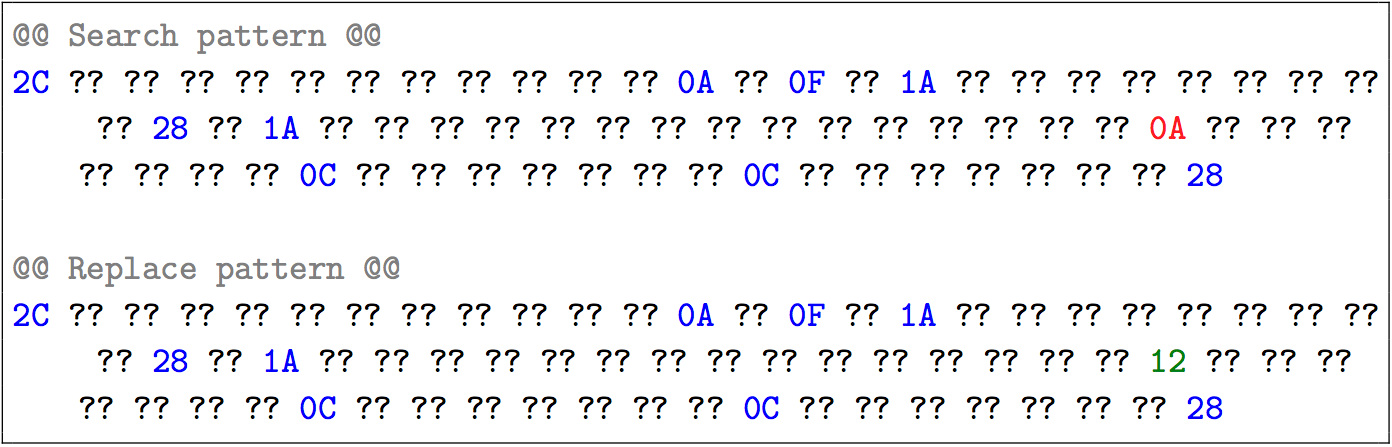
\includegraphics[width=0.47\textwidth]{n0.png}
  \caption{Search and Replace Pattern example \cite{neutze}}
  \label{n0}
\end{figure}
While the search pattern is used to locate the instruction of interest, the replace pattern is used to apply the changes. There is no bytecode added or removed in the process, but the control flow is altered to enforce a specific outcome of evaluations. This is achieved by manipulating single instructions of the bytecode by either changing its opcode or arguments. Since implementations never look the same, Patch Patterns have different bytecode patterns for changing the same functionality. All of the Patch Patterns are tried when patching and when a Search Pattern fits, the Replace Pattern is applied to change the instruction. The patterns applied by the chosen mode are shown when the manipulation has finished. There are seven Patch Patterns for the LVL, called N1 to N7. The following gives a detailed description on when the patterns are used, the targeted function and class, and resulting changes \cite{neutze}.\\
\b{Patch Pattern N1} and \b{Patch Pattern N2} are part of the auto and auto inverse mode.
These patterns target the verify() method inside the LicenseValidator class.
\begin{figure}[htbp]
  \centering
  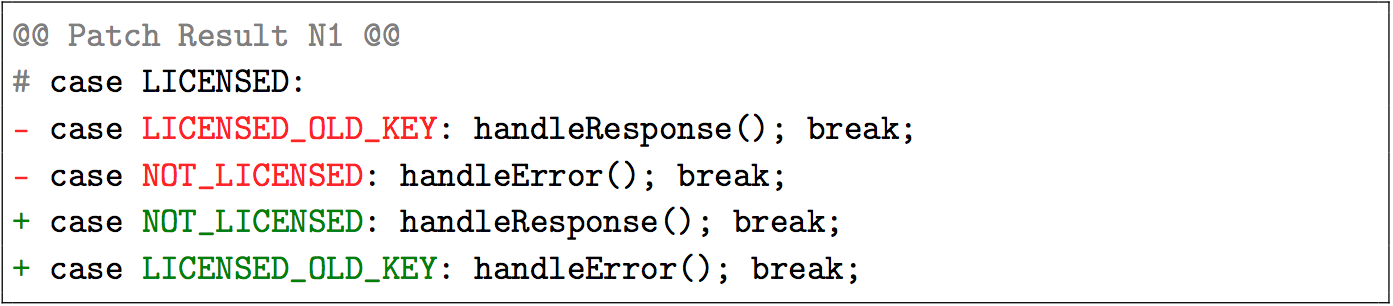
\includegraphics[width=0.47\textwidth]{n1.png}
  \caption{Result of Patch Pattern N1 \cite{neutze}}
  \label{n1}
\end{figure}
Patch Pattern N1 attacks the method's switch case by switching the cases for LICENSE\_OLD\_KEY and NOT\_LICENSED as seen in Figure~\ref{n1}.
This results in NOT\_LICENSED responses are being handled the same way as LICENSED responses and thus the result of the method always allows access.
\begin{figure}[htbp]
  \centering
  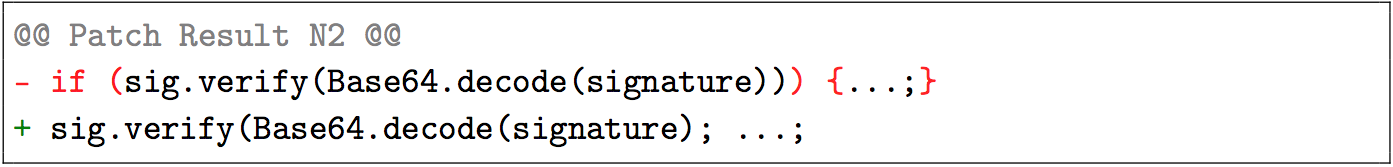
\includegraphics[width=0.47\textwidth]{n2.png}
  \caption{Result of Patch Pattern N2 \cite{neutze}}
  \label{n2}
\end{figure}
After Patch Pattern N2 (Figure~\ref{n2}) is applied, the signature is still verified but the evaluation is skipped and the former condition is always executed so the signature's validity is no longer required \cite{neutze}. \b{Patch Pattern N3} has two different variants, called N3 in the auto mode and N3i in the auto inverse mode.
Target of both patterns is the allowAccess() of APKExpansionPolicy and ServerManagedPolicy class.
Both Patch Patterns attack the same instruction but use opposing values.
While N3 bets on true as solution, N3i initiates the value as false (Figure~\ref{n3}) .
\begin{figure}[htbp]
  \centering
  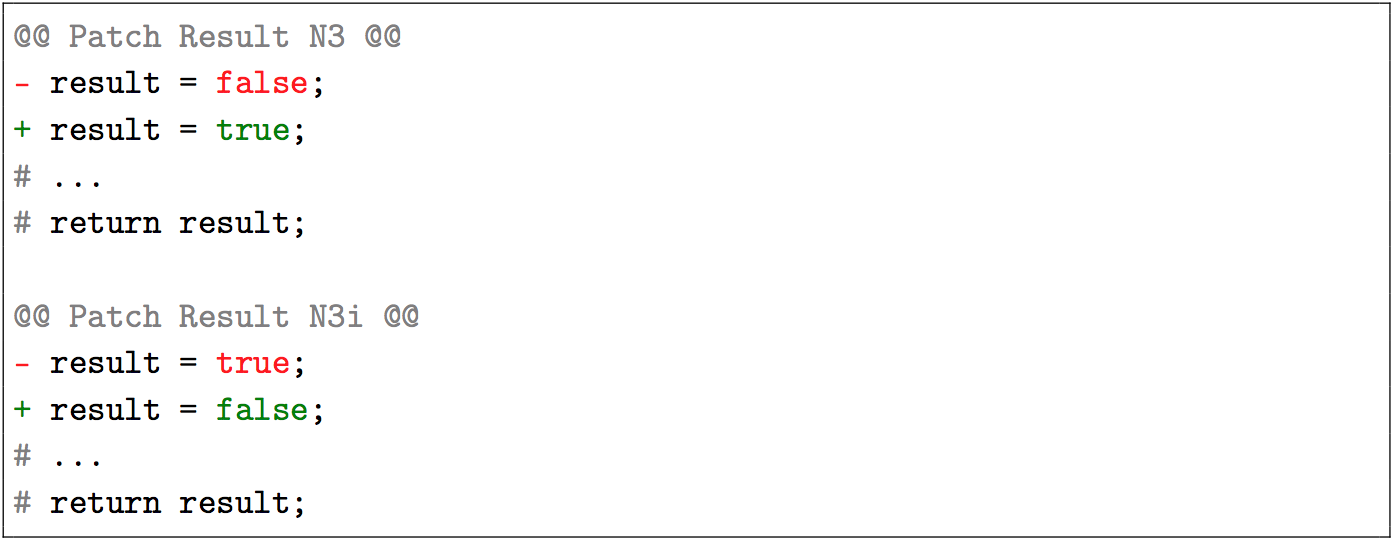
\includegraphics[width=0.47\textwidth]{n3.png}
  \caption{Result of Patch Pattern N3 \cite{neutze}}
  \label{n3}
\end{figure}
The result of the Patch Pattern is that the allowAccess() method is always successful since the result variable is initialized with the desired outcome. Since Lucky Patcher is not able to analyze or predict the code and the implementation is easily modified at this location, two opposing patterns are provided to cover both scenarios \cite{neutze}. \b{Patch Pattern N4} is applied by the auto and auto inverse mode and attacks the checkAccess() method inside the LicenseChecker class.
\begin{figure}[htbp]
  \centering
  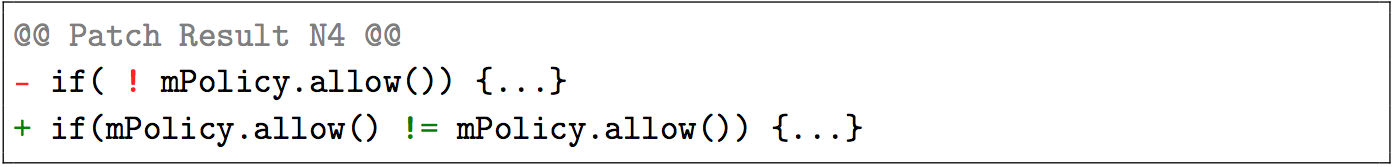
\includegraphics[width=0.47\textwidth]{n4.png}
  \caption{Result of Patch Pattern N4 \cite{neutze}}
  \label{n4}
\end{figure}
The pattern replaces the check for the validity of the policy of the response with an evaluation with itself as in Figure~\ref{n4}.
This way the result of the evaluation is always false and the condition code block is never executed \cite{neutze}.

\b{Patch Pattern N5} and \b{Patch Pattern N6} are part of the extreme mode.
Both patterns target the LicenseValidator class's verify() method.
\begin{figure}[htbp]
  \centering
  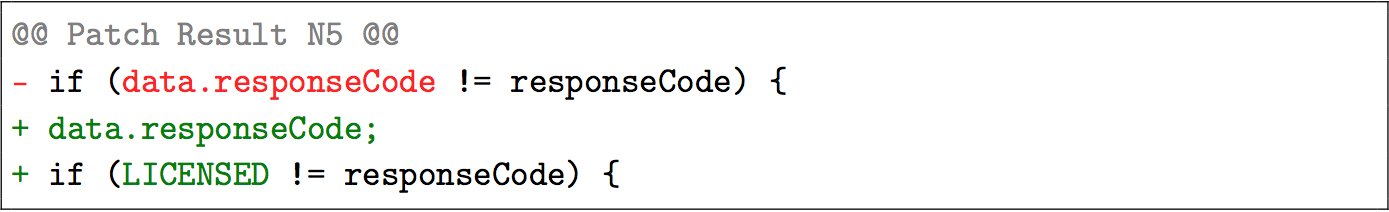
\includegraphics[width=0.47\textwidth]{n5.png}
  \caption{Result of Patch Pattern N5 \cite{neutze}}
  \label{n5}
\end{figure}
After applying Pattern N5, the parsed response code is no longer evaluated and instead the constant for LICENSED is used (Figure~\ref{n5}) \cite{neutze}.
\begin{figure}[htbp]
  \centering
  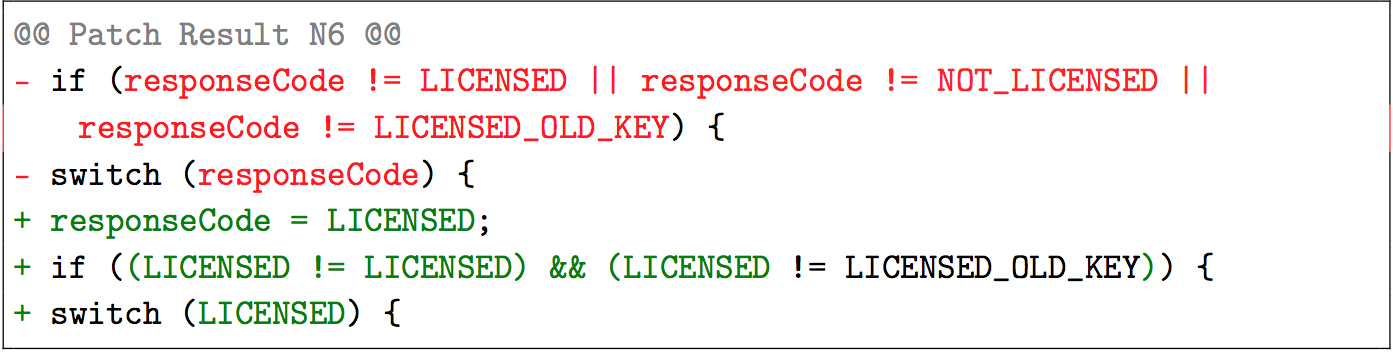
\includegraphics[width=0.47\textwidth]{n6.png}
  \caption{Result of Patch Pattern N6 \cite{neutze}}
  \label{n6}
\end{figure}
Patch Pattern N6 forces the evaluation to always be true. In addition,  the switch case returns always the same result since no longer the response code is used but a constant (Figure~\ref{n6}) \cite{neutze}.
\b{Patch Pattern N7} is applied when patching with the extreme mode.
It targets the onTransact() method of the ILicenseResultListener class.
\begin{figure}[htbp]
  \centering
  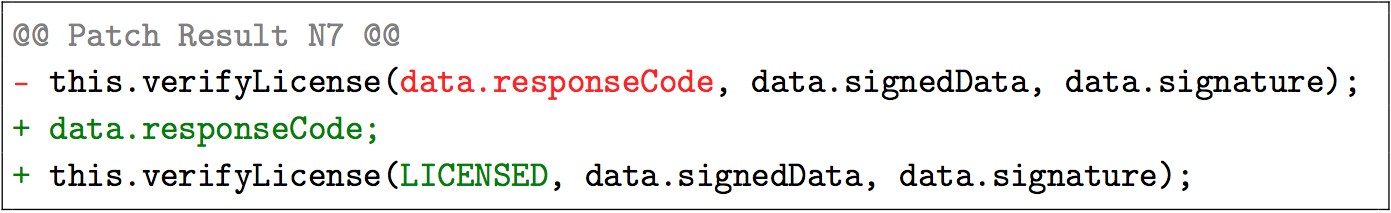
\includegraphics[width=0.47\textwidth]{n7.png}
  \caption{Result of Patch Pattern N7 \cite{neutze}}
  \label{n7}
\end{figure}
Figure~\ref{n7} shows the result of Patch Pattern N7.
The pattern ensures that the verifyLicense()'s parameter is set to LICENSED instead of the response code from the server \cite{neutze}. \\

Figure~\ref{LP} shows a screenshot of Lucky Patcher with all the modes and the performed cracking approach on one of our test apps. The figure shows that Lucky Patcher just tries out the pattern and hopes for a match. A general cracking approaches may be used to circumvent a specific protection by using custom recipes \cite{neutze}.

\begin{figure}[htbp]
  \centering
  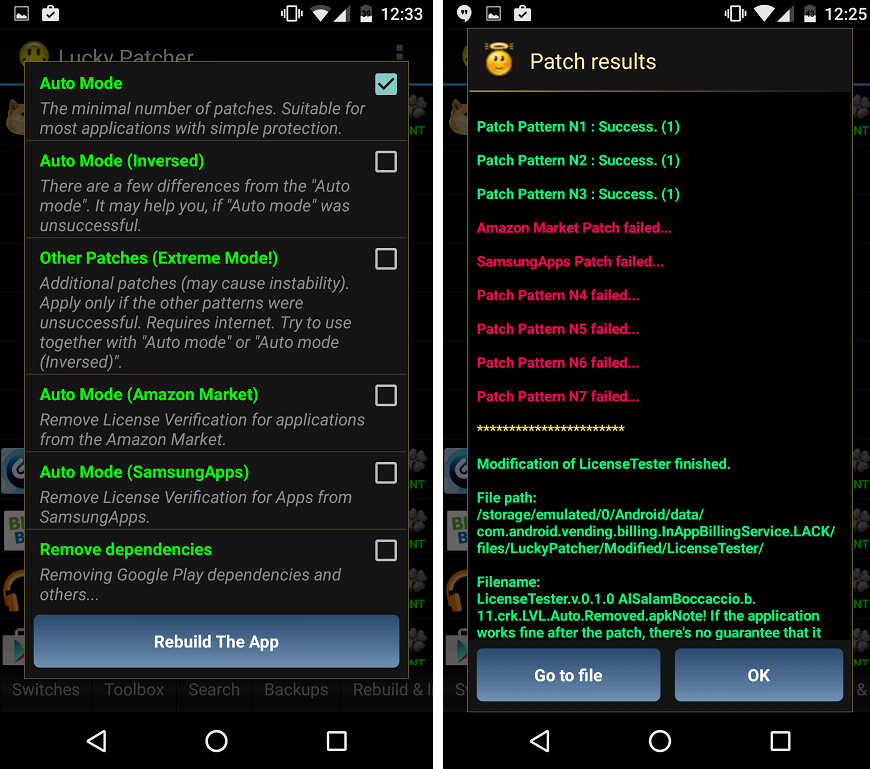
\includegraphics[width=0.47\textwidth]{LP.png}
  \caption{Lucky Patcher in action \cite{neutze}}
  \label{LP}
\end{figure}



\subsection{Cracking Applications using Typical Re-Engineering (example LVL and Amazon's DRM)}

Google's LVL was cracked years ago \cite{AT1}. While the easiest option to crack LVL is to use "Lucky Patcher" \cite{xAT2} and even non-savvy customers can crack and circumvent the protection with this tool, a more advanced attack requires some Android and reengineering knowledge by editing a single application itself by using the apktool. As outlined in \cite{AT1} the attacker is required to find the LicenseValidator.smali file that may be obfuscated, but typical structures and calls are still imaginable. Here and within the verify() method the attacker needs to look for a switch block. Values like 0x00 or 0x03 represent a valid license state, which links to the desired switch case. Ultimately the trick is to redirect the other cases (representing a failed license response) to the valid ones. By saving, recompiling and signing it, the app is cracked. 

Amazon uses a different approach to integrate their DRM protection by injecting their code into existing apps, regardless if DRM is requested or not, since the injected code is also used for communication purposes with the Appstore \cite{AT3}.
In 2014, Amazon's DRM was analyzed by \cite{xAT4} for the first time and our research revealed that there are essentially three function calls within the so-called kiwi-class, which need to be removed to disable the protection. In a recent review, it was discovered that the protection has been modified, but to our surprise, a new Boolean variable responsible for enabling or disabling DRM allows the deactivation of the protection within seconds for any protected app \cite{xAT7}. 
Since the protection is integrated by Amazon, developers can do almost nothing about it and depend on Amazon to improve their license protection. In theory, developers could integrate their own additional methods, but that is beyond the scope of this paper. Nevertheless, some options are presented in section \hyperref[defense]{Defense strategies}.


\subsection{Cracking Applications by Interception/Manipulation (example LVL)}

A more sophisticated attack solution is a universal crack that may be implemented using the Xposed Framework. It is usable with all default LVL implementations \cite{xAT4} if developers ignore Google's request to modify it. The Xposed framework works on rooted devices only and hooks itself into Android's Zygote process  responsible for launching all apps by forking child processes that inherit most of its loaded libraries \cite{AT4} . 

As analyzed and implemented by \cite{xAT4}, the attack works in a summarized way by intercepting the onTransact() method as well as the verify() method that is used internally by the LVL. The license response by the Google license server consists of six values including the actual (LICENSED) response code and the package name (by example). Moreover, a signature to allow the application to verify the response for any modifications is also added by the license server. On Android the whole response is supplied in a parcel that needs to be modified to circumvent the LVL. The parcel needs to be intercepted and altered, before executing the actual onTransact() method by changing the included response code to 0x00 (LICENSED) using our developed Xposed module. In addition, the signature has to be altered. Since the private key for creating the signature is known by Google only, a new public/private key pair needs to be created. The newly created private key can then be used to generate the valid signature for the changed response and both values, the new signature and the new public key, will replace the previous values before being forwarded to the verify() method. The app itself will receive the valid license response and continue as if everything is fine. \\


\section{DEFENSE STRATEGIES}
\label{defense}

Since this paper is focused on the attack options, defense methods are addressed only briefly and presented in a different paper by us; we present a short summary for the sake of completeness only. 

In general, we propose the use of native code for increased protection \cite{nils}, since reengineering is much more difficult and, according to our surveys of computer science students, many of these students are not used to ARM assembly and non-computer science students are not familiar with basic reengineering tools either. Moreover, available decompilers, like retdec.com, are often also not able to recover the entire code. In addition, native code can be protected and its obfuscation has been researched for decades. \\

For improved protection (cf. Lucky Patcher), it is sufficient to slightly modify the default LVL implementation by for example, renaming the packages and functions (also recommended by Google \cite{lvlOverview}). More advanced attacks using reengineering tools or interception cannot be prevented this way but aforementioned methods do buy some time. This issue applies to any protection because of the general insecurity of Android and related root access \cite{nils}, but the time factor can be optimized to the advantage of the developer (copyright holder) using various methods. For instance, we developed a native version of the LVL called "nLVL" \cite{chen} that is immune to Lucky Patcher, Xposed Framework and to typical proxy attacks due to its direct connection to the Google license servers while benefiting from the power of obfuscation methods for native code (e.g. static directive \cite{chen}). In addition, we investigated and developed methods to bind native and Java code together so that a separation of the app from the more secure native code is no longer easily possible and a separation will trigger certain protection methods thus render the application useless \cite{nils}.


\section{RELATED WORK}

There are various similar research works, but only few of them focus on similar topics like attacking libraries. In \cite{mulliner} Collin Mulliner et al. attacked the In-App-Billing Library by method call interception using their own libraries. In comparison we used the Xposed Framework for our LVL attacks instead. Most other related works focus on copyright protection for Android. One work, for example, focuses on the usage of smart-cards and application encryption using dynamic code loading for copy protection as presented by Shoaib et al. \cite{RW1}. Other researchers focus on improved copyright security by modifying opcodes to prevent the reengineering as described in the paper about "DIVILAR" by Wu Zhou et al. \cite{RW3}. Moreover, security companies provide external dongles to allow the execution of code in a more secure manner as outlined in e.g., \cite{RW2}.

\section{CONCLUSION}

Summarizing the status on Android in terms of copyright protection, the situation can be described as devastating. While many developers do not seem to be aware of the issues of reengineering in general, the available copyright protection used in major app markets is seriously deficient and can be circumvented by customers using cracking tools like Lucky Patcher. Our observation is shared by Eric Lafortune from GuardSquare, who collected some figures on the use of their obfuscation tools, stating, "We have collected some statistics on the protection of the top European banking apps. It seems that about 65\% use ProGuard, 15\% use DexGuard, and 20\% are unprotected [...] Considering that ProGuard only offers very basic protection (name obfuscation), most developers indeed seem to be unaware [of reengineering issues]" \cite{lafor}

In general, the situation on Android will not improve as long as Google provides access to the DEX file that is still included in current OAT formats (new format used by ART VM) \cite{xAT11} \cite{nils}.

\section{FUTURE WORK}

Since there are no additional, secure solutions available that are widely used, there is no imminent future work on the same topic of introducing cracking possibilties possible. Nevertheless, alternative solutions by other researchers as well as our own solutions may be re-evaluated in the future, while current evaluations of our solutions have already provided a significant improvement against existing copyright protection solutions.
%\end{document}  % This is where a 'short' article might terminate

%ACKNOWLEDGMENTS are optional
\section*{APPENDIX}

\section*{LEGAL}

Both companies - Google and Amazon - have been notified about the problems related to their license verification in 2015 and in early 2016. In addition, Google was notified about protection solutions and invited to participate in the project which brings native protection to a broad range of developers. Furthermore, any presented attacks are not described in great detail to prevent malicious usage right away. More information or source codes are available upon justified request. 

\section*{UNPUBLISHED WORKS}

While the 1st author's dissertation is submitted for review and currently not yet publicly available, other unpublished and used references are not accessible due to legal reasons. Upon justified request these works are available and can be requested from the 1st author.

\section*{ACKNOWLEDGMENT}

We would like to thank our former and current students Marius Muntean, Sebastian Schleemilch, Yixiang Chen, Jonas Raedle and Gabriel Michels that provided us input via their research works and theses, but were not involved in the actual writing of this paper. \\


% EINFÜGEN
\section*{ABBREVIATIONS}
\begin{acronym}[Bash]
 \acro{APK}{Application Package} 
 \acro{ART}{ART VM for Android by Google} 
  \acro{DEX}{Dalvik Executable} 
   \acro{DRM}{Digital Right Management} 
    \acro{JAR}{Java Archive} 
     \acro{LP}{Lucky Patcher}
 \acro{LVL}{License Verification Library}
 \acro{SDK}{Self Development Kit}
  \acro{OAT}{Ahead of time} 

\end{acronym}

%
% The following two commands are all you need in the
% initial runs of your .tex file to
% produce the bibliography for the citations in your paper.
% sigproc.bib is the name of the Bibliography in this case
% You must have a proper ".bib" file
%  and remember to run:
% latex bibtex latex latex
% to resolve all references
%
% ACM needs 'a single self-contained file'!
%
%APPENDICES are optional
%\balancecolumns
%\balancecolumns % GM June 2007
% That's all folks!
\begin{thebibliography}{99}
\bibitem{luckypatcherPage} ChelpuS, Lucky Patcher, \burl{http://lucky-patcher.netbew.com/}. Last access: 07-18-2016.
\bibitem{lvlRelease} E. Chu. Licensing Service For Android Applications, \burl{http://android-developers.blogspot.de/2010/07/licensing-service-for-android.html}, Last access: 07-18-2016.
\bibitem{lvlOverview} Android Developers, Licensing Overview, \burl{https://developer.android.com/
google/play/licensing/overview.html}, Last access: 07-18-2016.
\bibitem{lvlSetup} Android Developers, Setting Up for Licensing, \burl{https://developer.android.
com/google/play/licensing/setting-up.html}, Last access: 07-18-2016.
\bibitem{neutze} J. Neutze, Master's Thesis, "Analysis of Android Cracking Tools and Investigations into Countermeasures for Developers", unpublished.
\bibitem{chen} Master's thesis by Yixiang Chen, unpublished.
\bibitem{AT1}Justin Case, "[EXCLUSIVE] Report: Google's Android Market License Verification Easily Circumvented, Will Not Stop Pirates", \burl{http://www:androidpolice:com/2010/08/23/exclusive-report-googles-android-market-license -verification-easily-circumvented-will-not-stop-pirates}, Last access: 07-15-2016.
\bibitem{AT2}ComTech. "Kantar Worldpanel", \burl{http://www.kantarworldpanel.com/global/smartphone-os-market-share/}, Last access: 07-18-2016.
\bibitem{AT3}Amazon, "Publishing Android Apps to the Amazon Appstore". \burl{https://developer.amazon.com/public/support/submitting-your-app/tech-docs/submitting-your-app}, Last access: 07-18-2016.
\bibitem{AT4}Revo89, "Development tutorial", \burl{https://github.com/rovo89/XposedBridge/wiki/Development-tutorial}, Last access: 07-18-2016.
\bibitem{AT5}SaurikIT LLC, "Cydia Substrate", \burl{http://www.cydiasubstrate.com/}, Last access: 07-18-2016.
\bibitem{AT6}NowSecure, "Frida", \burl{http://www.frida.re/}, Last access: 07-18-2016.
\bibitem{AT7}SlideMe, "SlideLock", \burl{http://slideme.org/slidelock}, Last access: 07-18-2016.
\bibitem{AT8}Cedric Van Bockhaven, "Intercepting Android native library calls", \burl{https://cedricvb.be/post/intercepting-android-native-library-calls/}, Last access: 07-18-2016.
\bibitem{xAT2}ChelpuS, "Lucky Patcher", \burl{http://lucky-patcher:netbew:com/}, Last access: 07-15-2016.
\bibitem{xAT4} Marius Muntean, Master's thesis - Improving License Verification in Android, unpublished.
\bibitem{xAT7} Gabriel Michels, Jonas Raedle, TUM Android Practical Course - Workshop on Amazon DRM, unpublished.
\bibitem{addingLvl} Android Developers, Adding Licensing to Your App,\burl{https://developer.android.com/google/play/licensing/adding-licensing.html#lc-lcc}, Last access: 07-27-2016.
\bibitem{xAT11} Sebastian Schleemilch, Master's thesis, "Research and Analysis of Copy Protection Mechanisms for Android Apps, as well as Implementing a Sample Application", \burl{http://www:os:in:tum:de/fileadmin/w00bdp/www/Lehre/Abschlussarbeiten/MA_Schleemilch_Android_Copy_Protection:pdf}, Last access: 07-15-2016.
\bibitem{RW1}Muhammad Shoaib, Noor Yasin, Abdul G. Abbassi, "Smart Card Based Protection for Dalvik Bytecode - Dynamically Loadable Component of an Android APK", \burl{http://www.ijcte.org/vol8/1036-C040.pdf}. Last access: 07-18-2016.
\bibitem{RW2}Aktiv Soft JSC, "Guardant Code", \burl{http://www.guardant.com/products/all/guardant-code/}, Last access: 07-18-2016.
\bibitem{RW3}Wu Zhou, Zhi Wang, Yajin Zhou, Xuxian Jiang, "DIVILAR: Diversitying Intermedia Language for Anti-Repackaging on Android Platform", CODASPY 2014.
\bibitem{nils} Nils Kannengiesser, Dissertation, "Improving Copy Protection for Mobile Apps", in review / not published.
\bibitem{lafor} Email by Eric Lafortune by 06-24-2016, unpublished.
\bibitem{apktool}Connor Tumbleson, Ryszard Wisniewski, "A tool for reverse engineering Android apk files", \burl{https://ibotpeaches.github.io/Apktool/}, Last access: 07-18-2016.
\bibitem{mulliner}Collin Mulliner, William Robertson, Engin Kirda, "VirtualSwindle: An Automated Attack Against In-App", ASIA CCS, Japan 2014



\end{thebibliography}
\end{document}